\documentclass{article}
\usepackage[utf8]{inputenc}
\usepackage{hyperref}
\usepackage{amsmath}
\usepackage{amsfonts}
\usepackage{graphicx}


\title{SPhO Ten Year Series (TYS) with Solutions: 2020 Questions}
\author{
    Solutions available on Victoris\\
    \texttt{victoris.org}
    % new collaborators add your name and contact here!
}

\date{\today}

\begin{document}
\maketitle

\section{2020}
\subsection{Question 1}
A cylindrical rod has a radius of 1.0 cm and length 1.0 m. It is made up of two sections, each of length 0.5 m. The material of one section is zinc and that of the other section is copper. The end of the rod made of zinc is pivoted to a fixed point O. The rod is first held so that it is horizontal and then released. Determine the angular velocity of the rod when it is in the vertical position. (Densities: zinc: 7135 kg $\text{m}^{-3}$; copper: 8940 kg $\text{m}^{-3}$) [10]

\subsection{Solution 1}
Mass of the zinc rod $m_{zinc} = \pi r^2 l \rho_{zinc} = \pi (0.01)^2 (0.50) (7135) = 1.1208 \text{ kg}$ \\
Mass of the copper rod $m_{copper} = \pi r^2 l \rho_{copper} = \pi (0.01)^2 (0.50) (8940) = 1.4043 \text{ kg}$ \\
\\ Moment of inertia about pivot 
\begin{align}
	&I=I_{zinc} + I_{copper}\\
	&=\frac{1}{3} m_{zinc} l^2 + \left(\frac{1}{12} m_{copper} l^2 + m_{copper} (1.5l)^2\right) \text{ (by parallel axis theorem)} \\
	&= \frac{1}{3} 1.1208 (0.5)^2 + \left(\frac{1}{12} 1.4043 (0.5)^2 + 1.4043 (1.5(0.5))^2\right) \\
	&= 0.91258 \text{ kg m}^2
\end{align}
By conservation of energy, (rotational) kinetic energy + gravitational potential energy should be conserved.
\begin{align}
	\frac{1}{2} I \omega^2 &= m_{zinc}g \Delta h_{zinc} + m_{copper}g \Delta h_{copper} \\
	\frac{1}{2}(0.91258) \omega^2 &= (1.1208)(9.81)(0.25) + (1.4043)(9.81)(0.75) \\
	\omega &= 5.3542 \text{ rad s}^{-1}
\end{align}

\subsection{Question 2}
(a) A student is sitting on a swing which is swinging back and forth with a constant angular amplitude of 45°. The length of the swing is 5 m. A loudspeaker, placed at a short distance away from the swing, produces a sound with a constant frequency of 400 Hz. What are the maximum and minimum frequency of the sound heard by the student? (Speed of sound waves = 330 m/s) [5] \\
(b) A compound microscope contains two thin lenses of focal length 6.0 mm and 40.0 mm respectively. The lenses are separated by a distance of 200 mm. The final image is formed 250 mm away from the eye lens. Calculate [5] \\
(i) The distance of the object from the objective lens \\
(ii) The magnifying power of the microscope\\
\subsection{Solution 2}
(a) The maximum doppler shift occurs when the swing is moving at its highest speed, i.e., at the lowest point. By the principle of conservatio nof energy,
\begin{align}
	\frac{1}{2} mv^2 &= mgl \left(1-\cos 45^\circ \right)\\
	\frac{1}{2} v^2 &= (9.81)(5) \left(1-\cos 45^\circ \right)\\
	v &= 5.3603 \text{ms}^{-1}
\end{align}
Hence,
\begin{align}
	f_{max} & = \frac{v_{sound}+v}{v_{sound}} f = \frac{330+5.3603}{330} \times 400 = 406.50 \text{ Hz} \\
	f_{min} & = \frac{v_{sound}-v}{v_{sound}} f = \frac{330-5.3603}{330} \times 400 = 393.50 \text{ Hz}
\end{align}
\begin{figure}
	\centering
	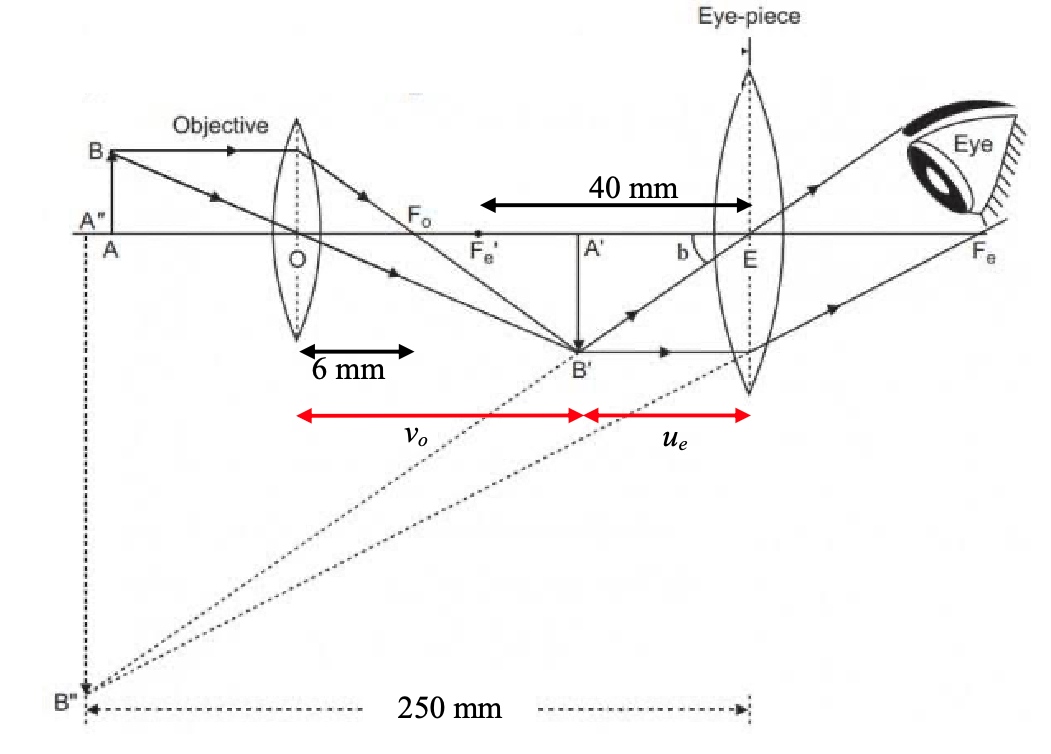
\includegraphics[width=\linewidth]{spho_book_TYS_images/2020q2.png}
\end{figure}
(b) 
\[f_o = 6 \text{ mm}\]
\[f_e = 40 \text{ mm} \quad v_e = -250 \text{ mm} \quad u_e = 200 - v_o \]
\begin{align}
	\frac{1}{u_e} + \frac{1}{v_e} &= \frac{1}{f_e} \\
	\Rightarrow	\frac{1}{200-v_o} + \frac{1}{-250} &= \frac{1}{40} \\
	\Rightarrow v_o &= 165.52 \text{ mm}
\end{align}
Hence,
\begin{align}
	\frac{1}{u_o} + \frac{1}{v_o} &= \frac{1}{f_o} \\
	\Rightarrow	\frac{1}{u_o} + \frac{1}{165.52} &= \frac{1}{6} \\
	\Rightarrow u_o &= 6.2257 \text{ mm}
\end{align}
\[u_e = 200-v_o = 200-165.52 = 34.480 \text{ mm}\]
Hence, magnification of eye lens $= \frac{250}{34.480} = 7.2506$ \\
And magnification of objective lens $ = \frac{165.52}{6.2257} = 26.587$ \\
Combined power of microscope $= 7.2506 \times 26.587 = 192.77 $
\subsection{Question 3}
One end of a thin conducting rod of length $l$ is pivoted to a fixed point. The rod has a resistance of $R$ and its two ends of the rod are connected to a resistor with resistance $R_0$. The rod is rotating with a constant angular velocity $\omega$ in a uniform magnetic field of flux density $B$. This direction of magnetic field is normal to the plane of rotation of the rod. [10]\\
(a) What is the emf induced in the rod? \\
(b) Determine the electric power developed in the resistor. \\
(c) Describe, with evidence, the origin of the electric power developed in the resistor.

\subsection{Solution 3}
3 (a) Induced emf $=B l v$
$$
=B l\left(\frac{1}{2} l \omega\right)
$$
$$
=\frac{1}{2} B l^{2} \omega
$$
(b) Power $=\frac{V^{2}\left(\frac{R_{o}}{R+R_{o}}\right)^{2}}{R_{o}}=\frac{\frac{1}{4} B^{2} l^{4} \omega^{2} R_{o}}{\left(R+R_{o}\right)^{2}}$ \\
(c) The electric power comes from the mechanical power input to sustain the circular motion of the rod which experiences an opposing torque due to the induced current.
The total electrical power dissipated is $=\frac{V^{2}}{R+R_{o}}=\frac{\frac{1}{4} B^{2} l^{4} \omega^{2}}{R+R_{o}}$
The induced current is $\frac{V}{R+R_{o}}=\frac{\frac{1}{2} B l^{2} \omega}{R+R_{o}}$
For each short length $d x$ of the rod located $x$ from the pivot, the torque is
$$
d \tau=x \cdot(B I d x)=B\left(\frac{\frac{1}{2} B l^{2} \omega}{R+R_{o}}\right) x d x=\frac{1}{2} \frac{B^{2} l^{2} \omega}{R+R_{o}} x d x
$$
Hence, total torque is
$$
\tau=\frac{1}{2} \frac{B^{2} l^{2} \omega}{R+R_{o}} \int_{0}^{l} x d x=\frac{1}{2} \frac{B^{2} l^{2} \omega}{R+R_{o}}\left(\frac{l^{2}}{2}\right)=\frac{1}{4} \frac{B^{2} l^{4} \omega}{R+R_{o}}
$$
Total mechanical power $=\tau \omega=\frac{1}{4} \frac{B^{2} l^{4} \omega^{2}}{R+R_{o}}$ which is identical to the electrical power developed.

\subsection{Question 4}
A free electron collides with a hydrogen atom which is in the ground state. After the collision, the hydrogen atom is excited and during the process of de-excitation, two photons are emitted. The wavelength of one of the photons emitted is 656.3 nm. The electron, after the collision, has de Broglie wavelength of 1.915 nm. [10] \\
(a) What is the wavelength of the other photon emitted during the de-excitation? \\
(b)What is the speed of the free electron before collision?

\subsection{Solution 4}
4 (a) The energy levels of the hydrogen atom are $E_{n}=-\frac{13.6}{n^{2}} \mathrm{eV}$. The photon of $\lambda=$ $656.3 \mathrm{~nm}$ is due to the transition from $n=3$ to $n=2$ as can be verified as follows: $\quad \frac{h c}{\lambda}=E_{3}-E_{2}=-13.6 \times\left(1.6 \times 10^{-19}\right)\left(\frac{1}{3^{2}}-\frac{1}{2^{2}}\right)=3.022 \times 10^{-19} \mathrm{~J}$ $\Rightarrow \quad \lambda=\frac{6.63 \times 10^{-34} \times 299792458}{3.022 \times 10^{-19}}=6.58 \times 10^{-7} \mathrm{~m}$ which is almost the same as the given value.
Hence, the other photon is emitted when the hydrogen atom de-excites from $n=2$ to $n=1$.
$$
\begin{gathered}
	\frac{h c}{\lambda}=E_{2}-E_{1}=-13.6 \times\left(1.6 \times 10^{-19}\right)\left(\frac{1}{2^{2}}-\frac{1}{1^{2}}\right)=1.632 \times 10^{-18} \mathrm{~J} \\
	\Rightarrow \quad \lambda=\frac{6.63 \times 10^{-34} \times 299792458}{1.632 \times 10^{-18}}=1.22 \times 10^{-7} \mathrm{~m}
\end{gathered}
$$
(b) Let the initial energy of the electron be $E$ and its energy loss when it collided with the hydrogen atom be $\Delta E$.
$$
\Delta E=13.6 \times\left(1.6 \times 10^{-19}\right) \times\left(\frac{1}{1^{2}}-\frac{1}{3^{2}}\right)=1.93 \times 10^{-18} \mathrm{~J}
$$
The momentum $p$ of the electron after collision is 
$$
p = \frac{h}{\lambda} = 3.4621 \times 10^{-25} 
$$
Hence, $E=1.93 \times 10^{-18} + \frac{p^2}{2m} = 1.9958 \times 10^{-18}$
$$
\begin{aligned}
	&\frac{1}{2} m v^{2}= 1.9958 \times 10^{-18} \\
	&v=2.09 \times 10^{6} \mathrm{~m} \mathrm{~s}^{-1}
\end{aligned}
$$
Since $v \ll c$, we are justified in neglecting relativistic effects.


\subsection{Question 5}
(a) An airplane flying horizontally with a constant speed of $540 \text{km h}^{-1}$ at a height of $1200 \text{m}$ fires a projectile horizontally in its direction of motion at a speed of $u \text{ m s}^{-1}$ relative to the plane. At this instant, a vehicle is at a point on the ground d km horizontally from the airplane. The vehicle is moving with a constant speed of $40 \text{m s}^{-1}$ on a horizontal road in the direction of motion of the plane. What must be the minimum value of d so that the projectile will hit the vehicle? If, at the instant when the projectile is fired, the value of d is 5 times its minimum value, what is the speed of the projectile when it hits the vehicle? [7]\\
(b) A satellite is orbiting the Earth 400 km above the equator. Its sense of revolution follows the rotation of the Earth. When the satellite is vertically above a point P on the equator, it will take a photo of the region around P. How many photos can the satellite take in 24 hours? [5] 
\subsection{Solution 5}
5 (a) $540 \mathrm{~km} \mathrm{~h}^{-1}=\frac{540}{3.6}=150 \mathrm{~m} \mathrm{~s}^{-1}$
The time of flight can be calculated using $1200=\frac{1}{2} g t^{2} \Rightarrow t=15.64 \mathrm{~s}$
Hence, change in displacement $=(150+u-40) \times 15.64=1721+15.64 u$
To hit the vehicle, $d=1721+15.64 u$
For minimum $d$, set $u=0$. Hence,
$$
d_{\min }=\mathbf{1 7 2 1} \mathbf{m}
$$
If $d=5 d_{\min }=8603 \mathrm{~m}$,
$$
\begin{aligned}
	&8603=1721+15.64 u \\
	&u=440 \mathrm{~m} \mathrm{~s}^{-1}
\end{aligned}
$$
And speed of projectile $=\sqrt{(440+150)^{2}+(9.81 \times 15.64)^{2}}=\mathbf{6 1 0} \mathbf{~ m} \mathbf{s}^{-1}$
(b)
$$
\begin{aligned}
	m r \omega^{2} &=\frac{G M m}{r^{2}} \\
	\omega^{2} &=\frac{G M}{r^{2}} \cdot \frac{1}{r} \\
	&=g \cdot\left(\frac{R}{r}\right)^{2} \cdot \frac{1}{r} \\
	&=9.80\left(\frac{6371}{6371+400}\right)^{2} \cdot \frac{1}{(6371+400) \times 1000} \\
	\omega &=1.132 \times 10^{-3} \mathrm{rad} \mathrm{s}^{-1}
\end{aligned}
$$
Angular velocity of Earth's rotation is $\frac{2 \pi}{86400}=7.27 \times 10^{-5} \mathrm{rad} \mathrm{s}^{-1}$
Hence, relative angular velocity is $1.132 \times 10^{-3}-7.27 \times 10^{-5}=1.059 \times 10^{-3} \mathrm{rad} \mathrm{s}^{-1}$
Hence, $T=\frac{2 \pi}{\omega_{\text {rel }}}=5931 \mathrm{~s}$
Since there are $86400 \mathrm{~s}$ in one day, no of photos taken is $\frac{86400}{5931}=14.6$ photos. 

\subsection{Question 6}
(a) A charged insulating sphere of radius R has a uniform positive charge density $\rho$ throughout its entire volume. A very narrow tunnel is drilled along the sphere’s diameter passing through the centre of the sphere. A charged particle of mass m carrying a charge $-q$ is placed at one end of the tunnel and released. Describe the subsequent motion of the charged particle. What is the speed of the particle when it passes through the centre of the sphere? [6] \\
(b) A particle P of mass m moves along a straight line joining two fixed points A and B. The particle is under the action of two forces $F_A$ and $F_B$. $F_A$ acts towards the point A and has magnitude $2\mu m d_A$ where $d_A$ is the distance of the point P from A. $F_B$ acts towards the point B and has magnitude $\mu m d_B$ where $d_B$ is the distance of the point P from B. Given that $\mu$ is a constant, show that the motion of P is simple harmonic. Deduce an expression for the period of motion. During the oscillation, the particle is instantaneously at rest at the mid-point of AB. What is the amplitude of the oscillation and what is the kinetic energy of the particle when it is at O, the point where it experiences zero net force? [6]

\subsection{Solution 6}
6 (a) At a distance $r$ from the centre of the sphere, where $r \leq R$, the gravitational field strength is given by
$$
E=\frac{\left(\frac{4}{3} \pi r^{3} \rho\right)}{4 \pi \varepsilon_{o} r^{2}}=\left(\frac{\rho}{3 \varepsilon_{0}}\right) r
$$
Hence, the force acting the $-q$ is
$$
F=-q E=-\left(\frac{q \rho}{3 \varepsilon_{o}}\right) r
$$
The acceleration is thus $a=-\left(\frac{q \rho}{3 m \varepsilon_{o}}\right) r$
Since the term in the bracket consists of constants only, the acceleration of the charge is directly proportional to its displacement from the centre of the sphere and in opposite direction to the displacement. Hence, the charge $-q$ will oscillate in simple harmonic motion with angular frequency $\sqrt{\frac{q \rho}{3 m \varepsilon_{o}}}$ and amplitude $R$.
The speed at the centre is thus given by $v=\omega A=R \sqrt{\frac{q \rho}{3 m \varepsilon_{o}}}$.
(b) Let $d$ be the distance between $\mathrm{A}$ and $\mathrm{B}$.
$$
\begin{aligned}
	F_{\text {net }} &=F_{A}+F_{s} \\
	&=-2 \mu m d_{A}+\mu m\left(d-d_{A}\right) \\
	&=\mu m\left(d-3 d_{A}\right) \\
	&=-3 \mu m\left(d_{A}-d / 3\right) \\
	\Rightarrow a &=-3 \mu\left(d_{A}-d / 3\right)
\end{aligned}
$$
Therefore, the particle P oscillates about the point $d_{A}=1 / 3 d$ with $\omega=\sqrt{3 \mu}$.
The period is $T=\frac{2 \pi}{\omega}=\frac{2 \pi}{\sqrt{3 \mu}}$.
$$
\begin{aligned}
	&\text { Amplitude }=\frac{d}{2}-\frac{d}{3}=\frac{d}{6} \\
	&E_{k} \text { at } \mathrm{O}=\frac{1}{2} m \omega^{2} A^{2} \\
	&=\frac{1}{2}(3 m \mu)\left(\frac{d}{6}\right)^{2} \\
	&=\frac{m \mu d^{2}}{24}
\end{aligned}
$$

\subsection{Question 7}
(a) A container, the volume of which is $8.0\times 10^{-3} \text{ m}^3$, contains an ideal gas at a pressure of $1.14\times 10^5 \text{ Pa}$ and temperature $T$. The lid of the container is opened, causing the gas to expand adiabatically until its pressure $1.01\times 10^5 \text{ Pa}$. This results in a slight decrease in the mass of the gas in the container. The lid is then closed and the gas in the container is allowed to return to its initial temperature. Under the new equilibrium condition, the pressure of the gas is $1.06\times 10^5 \text{ Pa}$. [6] \\
(i) What will be the volume of the gas left in the container under the initial equilibrium condition; i.e. at pressure $1.14\times 10^5 \text{ Pa}$ and temperature $T$? \\
(ii) What is the value of $\gamma$, the ratio of the molar heat capacity of the gas at constant pressure to that at constant volume? \\
(iii) State, with reasons, what is the atomicity of the molecules of the gas? \\
(b) One end of a copper rod, with diameter 2.0 cm and length 50.0 cm, is in good thermal contact with a hot bath maintained at 100 °C while the other end is immersed in a mixture of 200 g ice and 100 g water initially maintained at 0 °C inside a container whose thermal capacity is negligible. Both the copper rod and the container are well-lagged. How long does it take for the temperature of the mixture to rise from 0 °C to 20°C? [6] \\
(Thermal conductivitiy of copper $= 400 \text{ W m}^{-1} \text{K}^{-1}$ \\ 
Specific heat capacity of water $=4200 \text{ J kg}^{-1} \text{K}^{-1} $ \\
Latent heat of fusion of water $= 3.34\times 10^5 \text{ J kg}^{-1}]$) 
\subsection{Solution 7}
7 (a) Imagine that the gas initially trapped in the container can be divided into the red portion and the blue portion below, and the blue portion escaped to the surrounding when the lid is opened and the gas expanded adiabatically. It is given that the final temperature of the remaining gas is $T$ and the pressure is $1.06 \times 10^{5} \mathrm{~Pa}$.
insert diagram
Hence, by $p V=n R T$ to diagrams 1 and 3 ,
$$
\frac{p_{f}}{p} \cdot \frac{V}{V}=\frac{n_{f}}{n} \cdot \frac{T}{T} \Rightarrow n_{f}=\frac{1.06}{1.14} n=0.930 n
$$
That is, $0.930$ of the original gas remains in the container.
(i) If this remaining gas is compressed to $1.14 \times 10^{5} \mathrm{~Pa}$ and remains at temperature $T$, then its volume is (using Boyle's Law):
$$
V_{f}=0.930 \times 8.0 \times 10^{-3}=7.44 \times 10^{-3} \mathrm{~m}^{3}
$$
(ii) Consider the adiabatic expansion of the "red gas", and applying $p V^{\gamma}=$ cosntant to diagrams 1 and 2 ,
$$
\begin{aligned}
	&\left(\frac{V}{V_{f}}\right)^{\gamma}=\frac{p_{f}}{p} \\
	\Rightarrow &\left(\frac{8.0}{7.44}\right)^{\gamma}=\frac{1.14}{1.01} \\
	\Rightarrow \quad & 1.075^{y}=1.129 \\
	\Rightarrow \quad & \gamma=1.67
\end{aligned}
$$
(iii) The molar heat capacity of a monatomic ideal gas at constant volume is $\frac{3 R}{2}$ while that at constant pressure is $\frac{5 R}{2}$. Hence, $\gamma=\frac{5 / 2}{3 / 2}=\frac{5}{3}=1.67$. That is, the atomicity of the gas molecules is 1 .
7 (b) The heat transfer can be broken down into two stages:
Stage 1 : when the ice is melting. The two ends of the copper rod are maintained at $100{ }^{\circ} \mathrm{C}$ and $0^{\circ} \mathrm{C}$ in this stage.
Stage 2: after the ice has fully melted, the cold water is gradually heated $\mathrm{up}$ to $20{ }^{\circ} \mathrm{C}$.
We will calculate the time taken for each stage as follows:
$\underline{\text { Stage } 1}$
$$
\begin{aligned}
	&\frac{d Q}{d t}=-k A \frac{d \theta}{d x}=-400 \times \pi(0.01)^{2} \times \frac{0-100}{0.500}=25.13 \mathrm{~W} \\
	&t_{1}=\frac{m_{i c e} l_{f}}{d Q / d t}=\frac{0.200 \times 3.34 \times 10^{4}}{25.13}=2658 \mathrm{~s}
\end{aligned}
$$
$\underline{\text { Stage } 2}$
$$
\begin{aligned}
	&\frac{d Q}{d t}=-0.04 \pi\left(\frac{\theta-100}{0.500}\right)=m c \frac{d \theta}{d t} \\
	&\Rightarrow \quad d t=\frac{0.500}{0.04 \pi} \times 0.300 \times 4200 \times \frac{d \theta}{100-\theta} \\
	&\Rightarrow \quad t_{2}=5013[\ln (100-\theta)]_{20}^{0}=1119 \mathrm{~s}
\end{aligned}
$$
Hence, total time taken $=2658+1119=3777 \approx \mathbf{3 7 8 0} \mathbf{s}$

\subsection{Question 8}
(a) Two identical sound sources A and B which emit sound waves with frequency 256 Hz are initially side by side together with a stationary observer. Source A remains stationary with respect to the observer, while source B accelerates from rest with a constant acceleration of 0.5 m s-2 until it reaches a point P. After this, B continues to move with a constant velocity that it attains at the point P. When this happens, the observer finds that the frequency of sound coming from source B differs from that from source A by 8 Hz. What is the distance of the point P from the observer? (Speed of sound waves in air = 330 m s-1) [5] \\
\begin{figure}
	\centering
	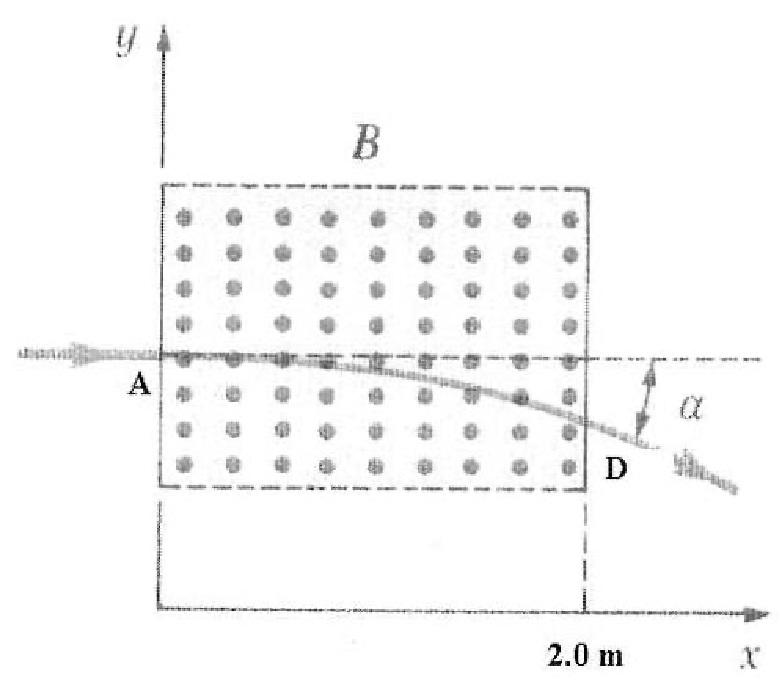
\includegraphics[width=\linewidth]{spho_book_TYS_images/2020q8}
\end{figure}
(b) A beam of protons with kinetic energy 10 MeV is travelling in the positive x-direction. It enters a magnetic field of magnitude 1.5 T and the direction of the magnetic field is the positive z-direction. The magnetic field extends from x = 0 to x = 2.0 m as shown in Fig. 1. Determine the angle $\alpha$ between the initial velocity vector of the proton bean and the velocity vector after the beam emerges from the magnetic field. [7] \\
\subsection{Solution 8}
8
(a) $f^{\prime}=f-8=248 \mathrm{~Hz}$
Hence, $248=256\left(\frac{c}{c+v}\right)$
$$
\begin{aligned}
	&31 c+31 v=32 c \\
	&v=\frac{1}{31} c=\frac{1}{31} \times 330=10.6 \mathrm{~m} \mathrm{~s}^{-1}
\end{aligned}
$$
By $v^{2}=u^{2}+2 a s$
$$
\begin{aligned}
	&10.6^{2}=2(0.5) s \\
	&s=\mathbf{1 1 3} \mathbf{m}
\end{aligned}
$$
(b) $\frac{1}{2} m v^{2}=1.6 \times 10^{-12} \Rightarrow v=\sqrt{\frac{1.6 \times 10^{-12} \times 2}{1.67 \times 10^{-27}}}=4.38 \times 10^{7} \mathrm{~m} \mathrm{~s}^{-1}$
Magnetic force provides the centripetal force:
$$
\begin{aligned}
	&\quad B q v=\frac{m v^{2}}{r} \\
	&\Rightarrow \quad r=\frac{m v}{B q}=\frac{1.67 \times 10^{-27} \times 4.38 \times 10^{7}}{1.5 \times 1.6 \times 10^{-19}}=0.305 \mathrm{~m}
\end{aligned}
$$
Therefore, since the radius of the trajectory of the proton is less than $2.0 \mathrm{~m}$, assuming that the magnetic field is of infinite extent in the $y$-direction (or more than $0.61 \mathrm{~m}$ from $\mathrm{A}$ in the negative $y$-direction), the proton will go through a semi-circular path before exiting the magnetic field again. Hence, $\alpha=180^{\circ}$.


\subsection{Question 9}
(a) Light with wavelength 122 nm is incident on the surface of a metal. The electrons, which are emitted with maximum kinetic energy, enters a magnetic field the direction of which is normal to the velocity vectors of these electrons. The flux density of the magnetic field is 5 x 10-5 T . These electrons are found to describe a circular path of radius 15.8 cm in the magnetic field. What is the work function of the metal? [5] \\
(b) Muons are particles which are created in the upper atmosphere via cosmic interactions. These particles travel vertically downward to the surface of the Earth at a speed of 0.995 c where c represents the speed of light in vacuum. When muons are at rest, they have a half-life of 1.56 $\mu$s. A muon counter is placed at the top of a mountain 2000 m high. The counter records 568 muons in 1 hour. \\
(i) According to classical concepts, what will be the number of muons counted in 1 hour if the counter is placed at the foot of the mountain? [2] \\
(ii) In a typical experiment, a counter placed at the foot of the mountain record 422 muons in 1 hour. Why does the result of this experiment differ so much from your result in part (i)? [2] \\
(iii) What is the “height” of the mountain according to muons? [1] \\
(iv) While the muons are travelling downward to the earth, another particle also travels in the same direction with speed 0.9995 c. What is the velocity of this particle in the muon’s inertial frame? [2]
\subsection{Solution 9}
9
$B q v=\frac{m v^{2}}{r}$ $\begin{aligned} \Rightarrow \quad r=\frac{m v}{B q} \\ 0.158 \end{aligned}=\frac{9.11 \times 10^{-31} \times v}{5 \times 10^{-5} \times 1.6 \times 10^{-19}}$ $v=1.39 \times 10^{6} \mathrm{~m} \mathrm{~s}^{-1}$ Hence, $K E_{\max }=\frac{1}{2} m v^{2}=8.77 \times 10^{-19} \mathrm{~J}$
$$
\begin{aligned}
	\text { Using } \frac{h c}{\lambda} &=\phi+K E_{\max }, \\
	\phi &=\frac{6.63 \times 10^{-34} \times 3.0 \times 10^{8}}{1.22 \times 10^{-7}}-8.77 \times 10^{-19}=7.53 \times 10^{-19} \mathrm{~J}
\end{aligned}
$$
(b) (i) Time taken to reach the ground level $=\frac{2000}{0.995 \times 3.0 \times 10^{8}}=6.70 \times 10^{-6} \mathrm{~s}$
$$
A=A_{o}\left(\frac{1}{2}\right)^{t / T_{V 2}}=568 \times\left(\frac{1}{2}\right)^{6.70 / .56}=29 \text { counts }
$$
(ii) This is due to time-dilation, i.e., in the reference frame of the muons, the time elapsed is $6.70 \times 10^{-6} / \gamma$, where $\gamma=(1-0.995)^{-1 / 2}=10.0$. So the time elapsed is $6.70 \times 10^{-7} \mathrm{~s}$ in the reference frame of the muons. The expected count rate should be
$$
A^{\prime}=A_{n}\left(\frac{1}{2}\right)^{0.677 / .56}=568 \times\left(\frac{1}{2}\right)^{0.67 / 1.56}=422 \text { counts }
$$
(iii) According to the muons, the height is $\frac{2000}{\gamma}=\mathbf{2 0 0} \mathrm{m}$
$$
\text { (iv) } \begin{aligned}
	u^{\prime} &=\frac{u-v}{1-u v / c^{2}} \\
	&=\frac{(0.9995-0.995) c}{1-0.9995 \times 0.995} \\
	&=0.819 c \\
	&=2.45 \times 10^{8} \mathrm{~m} \mathrm{~s}^{-1}
\end{aligned}
$$


\end{document}
